\documentclass{article}
\usepackage{fullpage}
\usepackage{amssymb}
\usepackage{amsthm}
\usepackage{amsmath}
\usepackage{ifsym}
\usepackage{array}
\usepackage{graphicx}
\setlength{\extrarowheight}{0.12cm}
\usepackage{polynom}
\usepackage{centernot}
\usepackage{enumerate}
\usepackage{caption}
\usepackage{parskip}
\usepackage[all]{xy}

%\usepackage{diagrams}
% Piecewise function
% \begin{displaymath}
%   f(x) = \left\{
%     \begin{array}{lr}
%       1 & : x \in \mathbb{Q}\\
%       0 & : x \notin \mathbb{Q}
%     \end{array}
%   \right.
% \end{displaymath} 
\newcommand{\st}{\mbox{ } \big | \mbox{ }}
\newcommand{\divides}{\mbox{ } \big | \mbox{ }}
\newcommand{\St}{\mbox{ } \bigg | \mbox{ }}
\newcommand{\iso}{\cong}
\newcommand{\normal}{\triangleleft}
\newcommand{\Z}{\mathbb{Z}}
\newcommand{\C}{\mathbb{C}}
\newcommand{\R}{\mathbb{R}}
\newcommand{\N}{\mathbb{N}}
\newcommand{\Q}{\mathbb{Q}}
\newcommand{\F}{\mathbb{F}}
\newcommand{\Aut}{\mbox{Aut}}
\newcommand{\Gal}{\mbox{Gal}}
\newcommand{\Tr}{\mbox{Tr}}
\newcommand{\diag}{\mbox{diag}}
\newcommand{\rank}{\mbox{rank}}
\newcommand{\im}{\mbox{im}}
\newcommand{\ws}{\mbox{ } \mbox{ } \mbox{ } \mbox{ } \mbox{ }}
\newcommand{\Arg}{\mbox{Arg}}
\newcommand{\of}{\circ}
\newcommand{\cyclic}[1]{\langle #1 \rangle}
\newcommand{\Matrix}[4]{\[ \left( \begin{array}{cc}
#1 & #2 \\
#3 & #4 \end{array} \right)\]}
\renewcommand{\sp}{\mbox{ }}
\renewcommand{\And}{\mbox{ and }}
\renewcommand{\H}{\mathbb{H}}
\renewcommand{\mod}{\mbox{ mod }}
\newcommand{\given}{\mbox{ } | \mbox{ }}


%: ----------------------- paths to graphics ------------------------

\ifpdf
    \graphicspath{{Figures/PNG/}{Figures/PDF/}{Figures/}}
\else
    \graphicspath{{Figures/EPS/}{Figures/}}
\fi


\begin{document}

\title{Annotated Bibliography}
\author{Lane McIntosh}
\maketitle
\tableofcontents

% Optimality in Early Sensory Systems
\section{Theoretical Neuroscience}
\subsection{Efficient and Predictive Coding}
\subsubsection{Atick 1992, Could Information Theory be an Ecological Theory of Sensory Processing?}

J.J. Atick identifies two sources of inefficiencies in information processing, 1) the unequal use of symbol values, and 2) statistical correlation between different symbols in a given message.  Consider a message $w = (m_1, \dots, m_l) \in M$ where each $m_i$ takes a value from a set of cardinality $N$.  Then
\begin{equation}
\underset{\mbox{statistical correlations between symbols}}{\underbrace{H(M) \leq \sum_{i = 1}^l \sum_{m_i = 1}^N p(m_i) \log_2 p(m_i)}} = \underset{\mbox{unequal use of $N$ symbol values}}{\underbrace{\sum_{i = 1}^l H(i) \leq \max_{\{p(m_i)\}} \sum_{i = 1}^l H(i)}} = C,
\end{equation}
where Atick defines $C$ to be the source capacity (note that this is quite different from channel capacity).  Each inequality represents the possible introduction of inefficiency into the source coding; the first inequality becomes an equality when symbol positions $m_1, \dots, m_l$ are statistically independent, and the second inequality becomes an equality when the $N$ values are used with equal frequency for each symbol. \\
\\
Defining redundancy (or total inefficiency) as
\begin{eqnarray}
R &=& 1 - \frac{H(M)}{C} \\
&=& \frac{1}{C} \left (C - H(M) \right ) \\
&=&  \underset{\mbox{unequal use of $N$ symbol values}}{\underbrace{  \frac{1}{C} \left (C - \sum_{i =1}^l H(i) \right ) }} +  \underset{\mbox{statistical correlations between the $l$ symbols}}{\underbrace{ \frac{1}{C} \left ( \sum_{i=1}^l H(i) - H(M) \right)}}
\end{eqnarray}
we can see how the 2 types of inefficiencies contribute to redundancy in the source code. \\
\\
Atick then references Laughlin, 1981 as an experimental verification that the nervous systems reduce the 1st kind of inefficiency (unequal use of $N$ symbol values).\\
\\
Introducing a simplified model of the retina where photoreceptor activity levels are mapped linearly and one-to-one onto retinal ganglion cells, Atick then derives the optimal filter.  Looking at this derived filter in Fourier space, we see that at low frequencies where noise is low the filter flattens the frequencies of the source (which for naturalistic stimuli is $1/|f|^2$) - i.e., it's a whitening filter.  Since whitening essentially removing the correlations in the stimulus, Atick interprets this optimal linear filter as the retina's method of removing the 2nd type of inefficiency (statistical correlations between symbols) from the visual world.\\
\\
Atick does however admit that, ``it is not clear in the retina what principle dictates the choice of the low-pass filter," since, although an optimal filter can be derived, a linear filter is not necessarily obtained when simply starting at the first principle that statistical correlations between symbols must be reduced.  Putting this in a modern context, this uncertainty is well justified; Xaq Pitkow and Markus Meister's 2012 paper for instance established that less than a quarter of the correlations present in naturalistic visual stimuli are reduced by the retina's linear filtering.  Instead, over half of the reduction in stimulus correlations is due to the nonlinear thresholding at the bipolar-retinal ganglion cell synapse.  As Xaq has mentioned, ``If the brain's computations could be carried out by linear filtering, and since the sum of many steps of linear filters is just another linear filter, we might as well not have a brain."\footnote{Pitkow, Xaq.  ``Efficient coding and beyond in the visual system."  The Stanford Center for Mind, Brain, and Computation Theoretical Neuroscience Colloquium Talk on Thursday, March 7.}




\subsubsection{Fairhall 2001, Efficiency and ambiguity in an adaptive neural code}
Fairhall et al. examine how the fly's retina adapts to changes in the visual stimulus statistics.  Although this adaptation allows for a more efficient encoding of the visual environment in the face of a neuron's limited dynamic range, adaptation inherently makes the meaning of a pattern of spikes ambiguous.  This paper investigates how these ambiguities are resolved.


\subsubsection{Baccus 2002, Fast and slow contrast adaptation in retinal circuitry}
Similar to the findings of Fairhall 2001 in motion sensitive H1 blowfly cells, Baccus and Meister observe fast and slow components of contrast adaptation in all retinal ganglion cells and certain bipolar and amacrine cells. \\
\\
Fast effects of a contrast increase included accelerated kinetics, decreased sensitivity, and a depolarization of the baseline membrane potential. Slow adaptation did not affect kinetics, but produced a gradual hyperpolarization. This hyperpolarization can account for slow adaptation in the spiking output of ganglion cells.


%\section{Predictive Coding}
\subsubsection{Hosoya 2005, Dynamic predictive coding by the retina}
This paper demonstrated {\it pattern adaptation} of retinal ganglion cell receptive fields.  The complex patterns they tested included
\begin{itemize}
\item full-field flicker vs. checkerboard of anti-correlated white noise
\item horizontal gratings vs. vertical gratings
\item time series where luminance values 60ms apart were anti correlated vs. same value.
\end{itemize}
They show that these adaptive changes are in the direction of rendering retinal ganglion cells more sensitive to novel stimuli, and argue that this adaptation of the RGC linear filters is due to activity-dependent synaptic plasticity between amacrine cells and RGCs.\\
\\
Barry Wark et al., 2007 summarizes this work nicely as well:
``This study explores adaptation to complex spatial or temporal correlations in salamander and rabbit retina, showing that the receptive fields of many RGCs change following stimulation with these correlated stimuli such that the response to novel stimuli is enhanced compared with the response to the adapting stimulus. The authors reject the hypothesis of fatigue of pattern matching cells in favor of a model of Hebbian plasticity at inhibitory amacrine-to-RGC synapses. This conclusion is intriguingly at odds with other studies that find adaptation in the retina to simpler correlations (mean, variance) in the absence of inhibitory transmission." \\
\\
Note that the paper does not deal with changes in contrast.  Kastner and Baccus 2011 demonstrated that under low contrast (i.e., high noise) regimes, RGC linear filters lengthen, leading to sensitization in many cells.

\subsubsection{Sharpee 2006, Adaptive filtering enhances information transmission in visual cortex}
From Barry Wark et al., 2007 review: ``This paper applies a novel information theoretic reverse correlation method [31] to obtain cat V1 receptive fields during viewing of a white noise stimulus and of natural movies. The receptive fields differed in the two cases in their low-pass properties, in such a way as to transmit similar low frequency power in the two cases. The information transmitted about the stimulus was determined to change on the order of $\sim$100 s.

\subsubsection{Nagel 2006, Temporal Processing and Adaptation in the Songbird Auditory Forebrain}
This paper demonstrates that adaptation in the avian auditory forebrain also have fast and slow components similar to those seen in the H1 motion sensitive cell in the blowfly (Fairhall 2001) and the salamander retina (Baccus 2002).

\subsubsection{Wark 2007, Sensory adaptation}
This is a review paper that discusses the presence of adaptation in early sensory systems at short and long timescales, and the evidence for whether the observed adaptation supports the efficient coding hypothesis.  One interesting point the paper makes is that, ``the change in coding strategy cannot be shorter than the time required for the system to 'learn' the new distribution."\\
\\
Here are some of the observations in sensory adaptation that Wark et al. mentions:
\begin{itemize}
\item Smirnakis et al., 1997, showed that retinal ganglion cells exhibit an adaptive change in firing rate when the variance of a flickering gaussian light stimulus changes
\item Brenner et al., 2000, demonstrated that the nonlinear gain function (in an LN model fitted to the fly motion sensitive neuron H1) adapted such that the scaling of the stimulus axis was normalized by the stimulus standard deviation and that this serves to maximize information transmission about the stimulus.  In essence, this is a whitening filter.
\item Fairhall et al., 2001, further showed that this maximization of information happens rapidly (in $\sim 100$ms) during continuous changes of the stimulus variance.
\end{itemize}
In addition to this fast contrast gain control adaptation, there is also a slower adaptive process that modulates the overall firing rate of retinal ganglion cells.  The take home message here is the distinction between contrast adaptation (slow, seconds), which essentially modulates the firing rate given the mean contrast to reduce Atick's 1st type of inefficiency, and contrast gain control (fast, $\sim 100$ms), which essentially changes the transfer function for a particular retinal location and spatial frequency to whiten the signal.
\begin{itemize}
\item Maravall et al. 2007 and Nagel \& Doupe 2006 have also shown evidence of filter and gain curve adaptation in rat barrel cortex (white noise stimulation of whiskers; covariance analysis used to estimate gain curves) and avian auditory cortex (broadband noise input; filters from a fitted LN model), respectively.
\item Dean et al. 2005 used Fisher information to demonstrate that the population of cells in inferior colliculus (responding to sound amplitudes) as a whole shifted responses to best encode the high probability sounds (although individual neurons had a variety of response changes during adaptation)
\end{itemize}
In a sense, classic studies on the remapping of sensory cortex in the absence of input from a particular region is an extreme example of how populations of neurons shift to encode high probability signals.  If suddenly there aren't any nonzero signals, it makes sense trivially from an information maximization sense to reallocate that neuronal population to a different region on the somatosensory map.
\begin{itemize}
\item Mante et al. 2005 found that adaptation of RGC filters to changes to the mean and variance (mean luminance and contrast) of drifting gratings occur independently.  They also examined natural scene statistics and found independence between luminance and contrast.
\item Bonin et al. 2005 examined how neurons in LGN respond to changes in the higher order statistics of random checkerboards and found no adaptation
\item Hosoya et al. 2005 generalized a previous finding of rate adaptation to the spatial scale of a flickering checkerboard to demonstrate adaptation to a variety of arbitrary spatiotemporal correlations in visual stimuli in RGCs and showed that the new filters that evolve after exposure to these correlations act to remove the correlations and so perform predictive coding
\item Sharpee et al. 2006 developed an information theoretic reverse correlation method that finds the stimulus dimensions that maximize mutual information between spiking responses and the stimulus - maximally informative dimensions - to estimate the receptive field under non-gaussian stimuli - i.e., for use with natural image stimuli.
\end{itemize}


\subsubsection{Meister 2008, Rapid Neural Coding in the Retina with Relative Spike Latencies}
This is a nice paper that 
\begin{itemize}
\item hypothesizes a rapid neural code (latency of the first spike) for conveying information about an image's structure,
\item provides evidence that this code contains more information about the stimuli than a neural code that uses spike count
\item demonstrates that the minimal model to generate a relative latency code requires RGCs to have input from ON and OFF bipolar cells, and
\item shows that by silencing ON bipolar cells, individual RGCs stop coding about half of the stimuli as predicted.
\end{itemize}
So the main results of the paper are that
\begin{enumerate}
\item the latency of a retinal ganglion cell's first spike relative to other RGCs first spike conveys information about an image's structure
\item and that input from both ON and OFF bipolar cells explains this
\end{enumerate}

\subsubsection{Pitkow 2012, Decorrelation and Efficient Coding in Retinal Ganglion Cells}
Historically the field of sensory coding has pointed to center-surround, biphasic spatiotemporal filtering in the retina as the primary mechanism of reducing the redundancy in natural scenes and decorrelating neural responses.  Pitkow and Meister investigate this claim by quantifying how each step of an LN model fit to salamander and macaque retina ganglion cells decorrelated natural images.  Surprisingly, they find that the nonlinearity contributes the most to decorrelating natural images. 

\begin{figure}
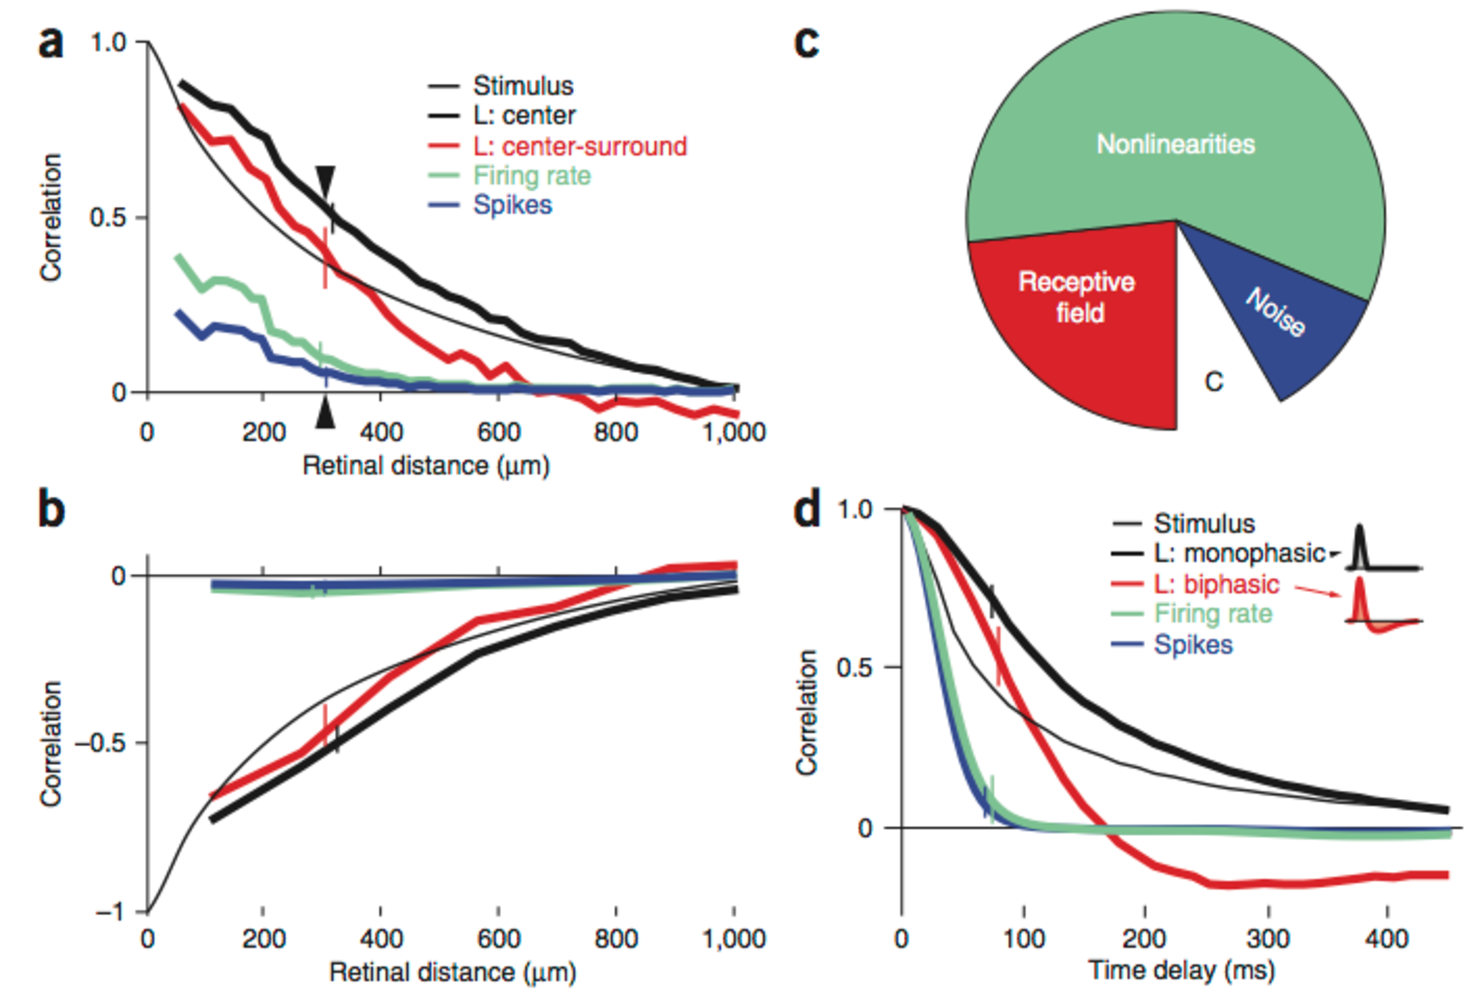
\includegraphics[width=\textwidth]{Pitkow2012_fig2_cropped.pdf}
\caption*{Figure 2 of Pitkow \& Mesiter, 2012}
\end{figure}
They then compute the optimal gain and threshold of a sigmoidal nonlinearity by assuming spike count distributions were Gaussian given the mean spike count (which is determined by the sigmoid nonlinearity), and then numerically optimizing bits/spike over the gain and threshold parameters.  Interestingly, if gain and threshold are estimated from the firing rates of salamander retinal ganglion cells, they fall within the nearly optimally efficient regime.
\begin{figure}
\centering
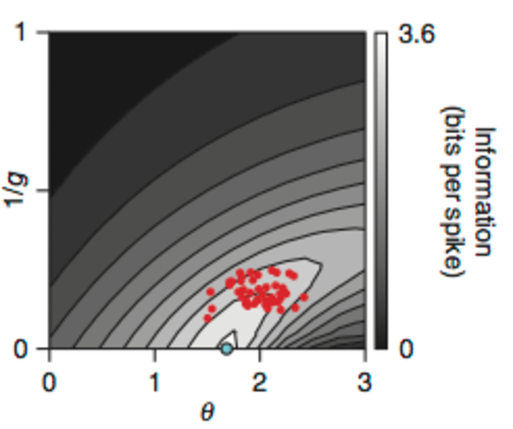
\includegraphics[width=0.2\textwidth]{Pitkow2012_fig5.pdf}
\caption*{Figure 5 of Pitkow \& Mesiter, 2012.  Red dots are salamander retinal ganglion cells.}
\end{figure}
It would be interesting to do a more fine grained analysis between and within different retinal ganglion cell types.  Presumably, the nonlinearity would strongly contribute to decorrelation between different cell types since direction-selective cells and object motion sensitive cells have different nonlinearities, for instance, while perhaps linear filtering is the best way of decorrelating cells of the same type.  Another thing to note is that the retinal ganglion cell receptive fields were measured using spatiotemporal white noise and then tested using natural images.  Since we know that these filters adapt dramatically, we may be dramatically underestimating the ability of linear mechanisms to decorrelate natural images.  A better approach would have been to use Maximally Informative Dimensions to measure the receptive fields under natural conditions.


\subsection{Energy Cost and Efficiency of the Brain}
\subsubsection{Laughlin 1998, The metabolic cost of neural information}
This paper measures the amount of ATP required in the blowfly retina to transmit a bit of information and compares it to Landauer's limit.  Laughlin et al. conclude that it costs $10^4$ ATP molecules to transmit a bit at a chemical synapse, and $10^6$ - $10^7$ ATP for graded signals in an interneuron or a photoreceptor, or for spike coding.  Since the hydrolysis of 1 ATP to ADP releases about 25 $kT$ (Landauer's limit is $kT$/bit), information transmission in neural networks is orders of magnitude ($2.5 \times 10^6$) more costly than the theoretical minimum.\\
\\
This paper also observes that in noise-limited systems, low capacity channels transmit information more efficiently.  This conclusion derived from their observation that the capacity of a neural signaling pathway is increased by adding more synapses.  This results in an exponential increase in the cost per bit of information transmitted as the bit rate increases.
 
 
\subsection{Methodologies}
\subsubsection{Strong 1998, Entropy and Information in Neural Spike Trains}
This publication from Bialek's group advocated the estimation of spike train entropies from the ``binary word'' approach.\\
\\
First, divide up spiketrain into non-overlapping segments of $T$ duration. Then choose some bin width $\Delta t$ such that a maximum of one spike appears in each bin.  Typically $\Delta t \approx 2$ ms, $T \to \infty$ approximated by taking 30 ms $< T <$ 100 ms and extrapolating.  For  approximately $T < 20$ ms the information rate (bits/s) increases linearly as $T$ becomes smaller.  Estimating the entropy for various $T < 20$ ms allows for linearly extrapolating the entropy in the $T \to \infty$ limit.



% Physics of Information and Inference in Physics
\section{Information Theory and Statistical Mechanics}

\subsection{Statistical Physics as Inference}
\subsubsection{Jaynes 1957, Information Theory and Statistical Mechanics I}
Rather than viewing statistical mechanics as its own separate physical theory, we should view statistical mechanics as a form of statistical inference.  Central to this shift in perspective is the idea that maximum entropy models are the least biased models that take into account our experimental constraints.

\subsection{Physics of Information}
\subsubsection{Still 2012, Thermodynamics of Prediction}
``All systems perform computations by means of responding to their environment."  In particular, how well systems respond to their environment - quantified by how much a system's dynamics predict future environmental driving signals - determines the physical dissipation of the system as it's driven by the environment.  In a sentence, information processing inefficiency is equivalent to thermodynamic inefficiency.
\begin{equation}
\beta \langle W_{\rm diss} [x_t \to x_{t + 1}] \rangle = I[s_t; x_t] - I[s_t; x_{t + 1}],
\end{equation}
where $s_t$ is the state of the system (for instance, the velocities and positions of gas molecules) at time $t$, $x_t$ is the environmental driving signal (for instance, the position of a piston) at time t, and $\beta = 1/k_B T$. \\
\\
This equality holds when the dynamics of the system are modeled by discrete time Markovian conditional state-to-state transition probabilities, $p(s_t \given s_{t - 1}, x_t)$.  The paper also assumes that the system begins in thermodynamical equilibrium at time $t = 0$, and that a change in the external driving signal $x_0 \to x_1$ forces the system out of equilibrium.


% Descriptions of Nervous Systems
\section{Observations from Experimental Neuroscience}
\subsection{Observations about Early Visual Systems}

\subsubsection{Hubel 1988, Segregation of Form, Color, Movement, and Depth}
This paper discusses the parallel pathways of visual information that are functionally distinct.  In particular, the magnocellular pathway (originating in parasol retinal ganglion cells) is sensitive to depth and movement, while the parvocellular pathway (originating in midget RGCs) is sensitive to form and color. \\
\\
The midget and parasol cells that comprise the parvo and magno cellular pathways in the retina, respectively, differ in color selectivity, contrast sensitivity, spatial resolution, and temporal properties.  Specifically, \\
\begin{tabular}{|c|p{4.5cm}|p{3.5cm}|c|c|} \hline
 	   & color selectivity & contrast sensitivity & spatial resolution & temporal properties \\ \hline
 parvo & typically color-opponent (e.g. center R, surround G) & higher contrast & sharper resolution & slower and more persistent \\ \hline
 magno & color-blind & more sensitive to low contrast (saturated at 10-15\%) & poorer resolution & faster and more transient \\ \hline
\end{tabular}

This raises an important point: when I'm using black and white stimuli, I may only be getting responses from parasol RGCs. 



\subsection{Noise in Neural Systems}

\subsubsection{Stevens 1968, Synaptic noise and other sources of randomness in motoneuron interspike intervals}
Poisson noise in spike trains assuming a rate code is on the order of 10\% the mean interval length.  This noise is due to synaptic noise originating from the temporal and spatial summation of PSPs.\\
\\
Calvin and Stevens ruled out noise in the mechanism converting synaptic currents into spike trains as a primary source of neural noise.\\
\\
Synaptic noise (fluctuations in membrane potential on the order of 2 mV peak to peak that vary quite a bit from cell to cell) could include 1) asynchronous arrival of PSPs, 2) spontaneous mini EPSPs, 3) thermal noise across the membrane impedeance ($~ k_B T/C$), and 4) shot noise from ions moving through the membrane.  But the primary source is the temporal and spatial summation of (1).  Fluctuations in the membrane potential due to thermal noise is $< 5 \mu V$ and fluctuations due to shot noise of ion movements is $< 1 \mu V$. \\
\\
Of course, if we don't believe the rate model, then reason (1) is not noise at all.


\subsection{Activity-dependent plasticity}
\subsubsection{Lanahan 1998, Immediate-early genes and synaptic function}
This is a brief overview of how immediate-early genes were first discovered, the scope of their influence on neurons, and four possible mechanisms that could describe why immediate-early genes tend to be localized at the synapse.\\
\\
Following work that suggested long-term memory required new protein synthesis, it was discovered that rapid mRNA synthesis (in addition to new protein synthesis) was also required for long-term plasticity.\\
\\
Immediate early genes like {\it{c-fos}} were originally found in assays looking at gene over-expression in neurons following seizures.\\
\\
One particularly interesting immediate early gene, {\it{zif268}}, was induced in hippocampal neurons by the same synaptic stimuli that induce LTP.  The induction of both LTP and {\it{zif268}} mRNA was dependent on activation of NMDA receptors and had the same threshold for stimulus intensity.  It seems that most neuronal IEG mRNAs are induced in response to NMDA receptor activation.  Does this suggest that neurons can change synaptic weights and otherwise alter information transmission by extracting information from sub-action-potential-threshold membrane potential voltages (i.e. even subthreshold NMDA current)? \\
\\
Scope of IEGs: Neuronal immediate early genes encode growth factors and proteins involved in signal transduction, transcription, cytoskeletal rearrangement, and metabolism (metabolic enzymes).  It is thought that IEGs may directly modify synaptic function as well, and IEGs tend to be localized at the synapse.  The authors expect that IEGs will contribute directly to synaptic plasticity by regulating the structure, signal transduction capability, or spatial localization of critical receptors.


\subsection{Feedback Connections}
\subsubsection{Sillito 2006, Always returning: feedback and sensory processing in visual cortex and thalamus}
Feedback connections are ubiquitous throughout the brain; for instance, only 10\% of the excitatory connections to the LGN are feedforward inputs from the retina.  The lion's share of inputs to LGN come from V1 and other higher areas of cortex, including MT.\\
\\
This review article explores feedback connections from MT to LGN and V1 that are thought to be involved in visual perception.\\
\\
Interaction between V1 and LGN:
\begin{itemize}
\item feedforward from LGN to layers 4 and 6 of V1
\item 30\% of LGN inputs are feedback from layer 6 of V1
\item feedback from V1 excites distal dendrites of LGN relay cells and inhibitory interneurons
\end{itemize}
MT has feedback connections to the V1 layer 6 cells that feedback to LGN.  This, together with the observation that layer 6 cells seem to modulate the cells in layer 4, leads the authors to speculate that layer 6 cells serve as a ``gatekeeper" of retinal input to the visual system.\\
\\
Affects of feedback on LGN cells:
\begin{itemize}
\item modulates strength of center-surround interaction for moving stimuli, in particular making surround antagonism stronger (lowering average firing rates of LGN cells and making them relatively more sensitive to shorter bars)
\item increases sensitivity to differences in grating orientation between center and surround (again only in the case of moving stimuli, not stationary flashing stimuli)
\end{itemize}










\end{document}